\documentclass[11pt]{report}
%\usepackage[german]{babel}

%(Rust) Code Snippets
\usepackage{minted}
\usemintedstyle{borland}

\setminted{
framesep=2mm,
fontsize=\footnotesize,
linenos
}
%\usemintedstyle{trac}

%table cells
\usepackage{makecell}

%chapter style
\usepackage{titlesec}
\titleformat{\chapter}{\normalfont\huge\textbf}{\thechapter.}{20pt}{\huge\textbf}


%Graphs
\usepackage{pgfplots}
\usepackage{subcaption} % For subfigures
\pgfplotsset{width=15cm,height=7.5cm,compat=1.9}
\usepgfplotslibrary{external}
\tikzexternalize
\usetikzlibrary{external}
\tikzexternalize % activate!

%CSV files
\usepackage{filecontents}

% For adjusting margins locally
\usepackage{changepage}

%Definitions
\usepackage{amsthm}
\usepackage{mdframed}

\NewDocumentCommand\newmdtheoremenvnonumber{O{} m m }{%
  \newtheorem*{#2}{#3}
  \BeforeBeginEnvironment{#2}{%
     \begin{mdframed}[#1]}%
  \AfterEndEnvironment{#2}{%
     \end{mdframed}}%
}

\newmdtheoremenvnonumber{mydefinner}{\mydeflabel}
\newcommand{\mydeflabel}{}
\newenvironment{mydef}[1]
 {\renewcommand\mydeflabel{#1}\begin{mydefinner}}
 {\end{mydefinner}}

\newcommand{\attribution}[1]{\textup{(#1)}}



%Citations
\usepackage[style=authoryear, backend=bibtex, urldate=long, sorting=none, defernumbers=true,autocite=superscript]{biblatex}
\addbibresource{refs.bib}
\usepackage{csquotes}


%Math Library
\usepackage{amsmath}

%Images Library
\usepackage{float}
\usepackage{graphicx}
\graphicspath{ {./images/} }

%General Layout
\usepackage{geometry}
\geometry{
    a4paper,
    left=20mm,
    right=20mm,
    top=30mm,
    bottom=30mm,
%    total={6in, 8in}
}
% To adjust figure placement
\usepackage{adjustbox}


%Background image
\usepackage[pages=some]{background}

%Liks of TOC
\usepackage{hyperref}
\usepackage{lstmisc}
\usepackage{holtxdoc}
\usepackage{pgfregressiontest}
\usepackage{hhline}

\hypersetup{
    colorlinks,
    linkcolor={blue!50!black},
    citecolor={blue!50!black},
    urlcolor={blue!80!black}
}


\backgroundsetup{
scale=1,
color=black,
opacity=1,
angle=0,
contents={%
\hspace*{13.5cm}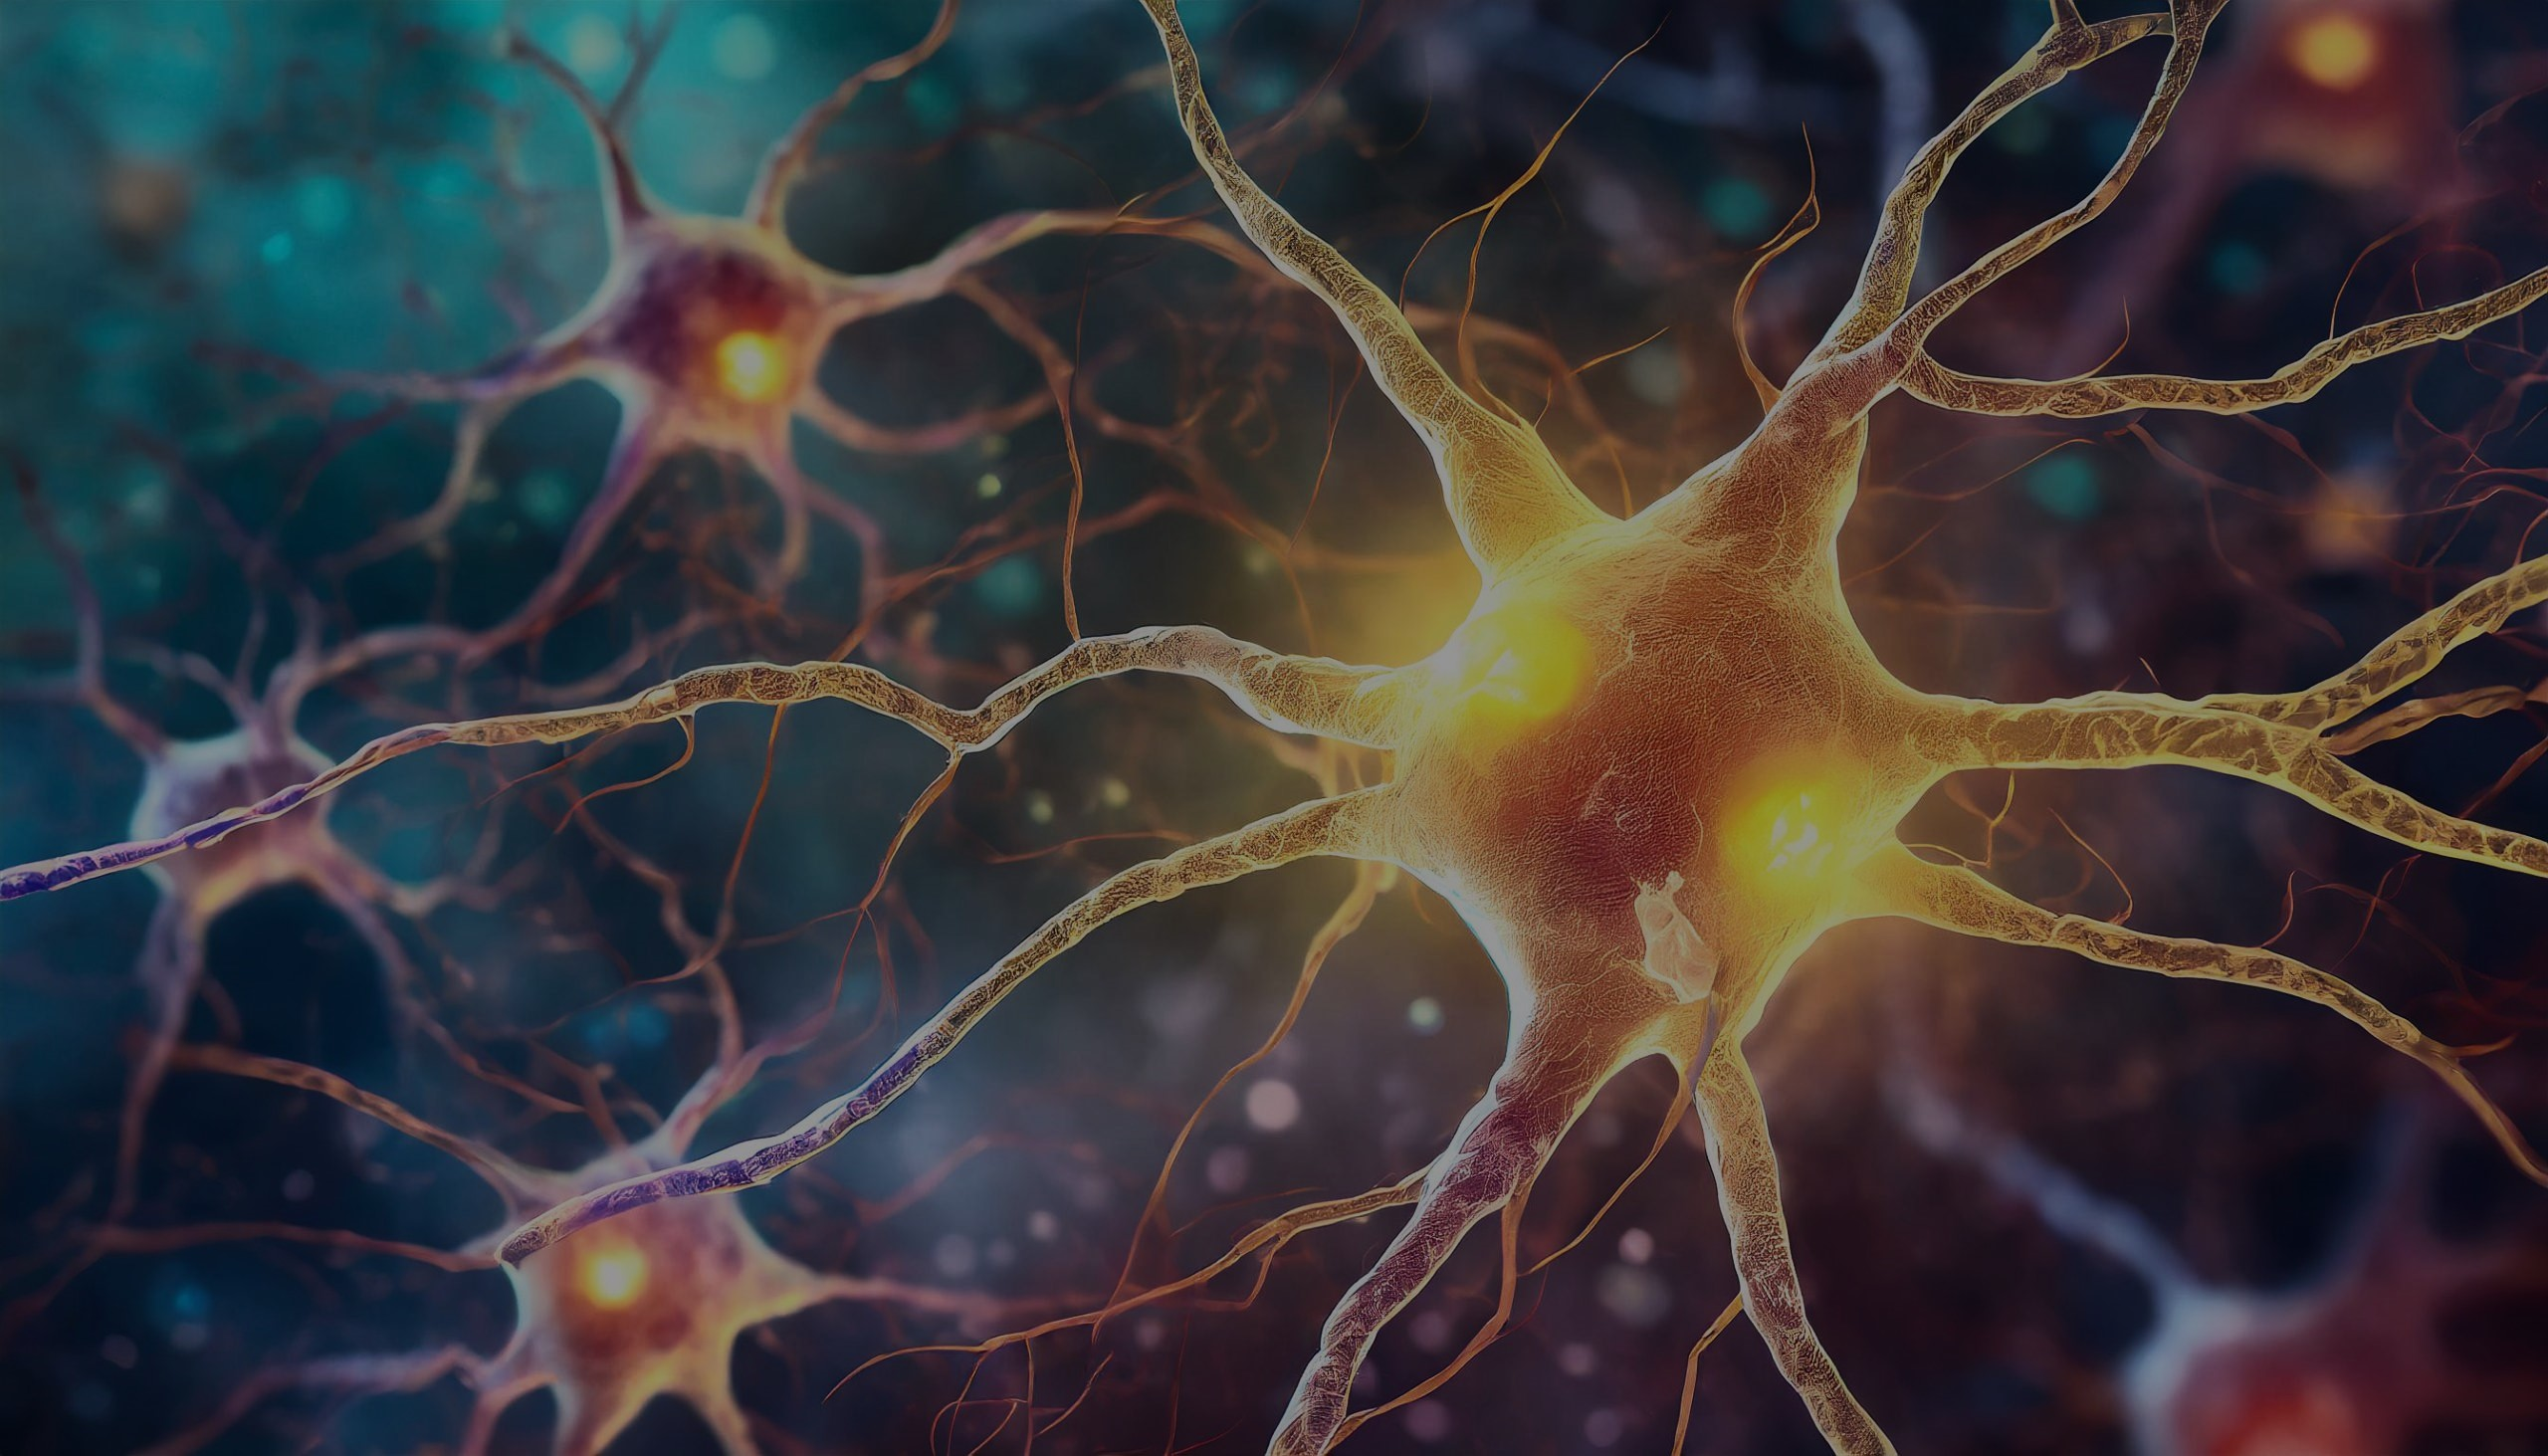
\includegraphics[width=3\paperwidth,height=\paperheight]{abstract_neurons3}
  }%
}


\begin{document}
    \pagenumbering{gobble}
    \begin{titlepage}
        \BgThispage
            \color{white} {
                \begin{center}
                    \Large \textsc{Matura Thesis}\\Kantonsschule Hohe Promenade\\
                    \rule[0.1cm]{15.8cm}{0.1mm}\\
                    \vspace{3cm}
                    \Huge \textbf{ \textsc{How can you develop \\Evolutionary Neural Networks which \\learn to play Board Games?}}\\
                    \vspace{0.8cm}
                    \Large \textit {Implementation and Study of\\ Evolutionary Neural Networks inspired\\ by the NEAT Algorithm}\\
                \end{center}
                \vspace{3cm}
                \rule[0.1cm]{15.8cm}{0.1mm}\\
                \vspace{9cm}\\
                \begin{minipage}[t]{0.47\textwidth}
                \large\textbf {Thesis By:}\\
                \end{minipage}
                \hfill
                \begin{minipage}[t]{0.47\textwidth}\raggedleft
                \large\textbf {Lucien Kissling 6e}\\
                \end{minipage}
                \begin{minipage}[t]{0.47\textwidth}
                \large \textbf {Year:}\\
                \end{minipage}
                \hfill
                \begin{minipage}[t]{0.47\textwidth}\raggedleft
                \large \textbf {2025}\\
                \end{minipage}
                \begin{minipage}[t]{0.47\textwidth}
                \large \textbf {Supervisor:}\\
                \end{minipage}
                \hfill
                \begin{minipage}[t]{0.47\textwidth}\raggedleft
                \large \textbf {Timo Schenk}\\
                \end{minipage}
                \begin{minipage}[t]{0.47\textwidth}
                \large \textbf {Co Examiner:}\\
                \end{minipage}
                \hfill
                \begin{minipage}[t]{0.47\textwidth}\raggedleft
                \large \textbf {Dr. Arno Liegmann}\\
                \end{minipage}
                \vfill
            }
        \clearpage
    \end{titlepage}
    \pagenumbering{arabic}
    \setcounter{page}{2}
    \tableofcontents
    \chapter{Introduction}\label{ch:introduction}
    \section{Preface}\label{sec:preface}
    Ever since I got into computer science a few years ago, I was fascinated by the idea of algorithms that solved various problems.
    Therefore, I participated in the SOI (Swiss Olympiad in Informatics) where we were taught everything about developing and programming algorithms and their data structures.
    \\ \\
    In recent years although, a new field of computer science has gained a lot of attention, where these algorithms are not programmed by humans, but evolved by a computer.
    This field called machine learning immediately got my excitement and two years ago a friend of mine and I had our first practical experience with it.
    We developed a simple neural network, which helped us predict the color of a lego brick in front of a color sensor based on the RGB values in various lighting conditions.
    \\ \\
    A neural network (NN) forms the basis of most machine learning models and I will therefore explain it in much detail in the following chapters.
    In simple terms however, a NN is a strongly simplified artificial model of the human brain consisting of an interconnected web of neurons through which information flows and gets computed.
    \\ \\
    Although the NN we developed two years ago already learned on its self, we still had to provide and label data for it to learn from.
    This meant that we had to manually scan the RGB values of the lego bricks and assign them the color they represented.
    In this case, this was the most efficient solution, however there are cases where you train a model where such data is unavailable or you simply want them to develop their own approach for a problem without predefined solutions.
    That is how I got to my matura thesis, which aims to develop such ML models that learn without labeled data with and use those to learn board games.

        \section{Thesis Statement}\label{sec:thesis-statement}
    This thesis will explore the field of neural networks (NNs) that learn without data provided by humans, which is called unsupervised learning.
    The solution this Thesis will focus on are evolutionary neural networks (ENNs), a combination of neural networks and evolutionary competition.
    \\ \\
    In this thesis, I develop my own simplified implementation of ENNs and then train them on some board games.
    The research effort consists of testing the ENN algorithm with different Parameters and Features to see how well it can learn to play the games in different configurations.
    My approach also draws inspiration from the NEAT Algorithm developed by Kenneth O. Stanley and Risto Miikkulainen in 2002, where the NNs start minimally in the first generation and then develop complexity over time.\footcite[p.105-106]{Neat_02}
    The first game I will train the ENNs on is Nim, a simple game where two players take turns removing matches from different stacks.
    \\ \\
    In specific, this Thesis aims to answer following questions:
    \begin{itemize}
        \item How can you develop evolutionary neural networks (ENNs) that learn to play board games?
        \item How do different parameters and features of ENNs affect the learning process?
        \item How does this implementation of ENNs compare to other Machine Learning Algorithms?
    \end{itemize}
    \chapter{Background}\label{ch:background}
    \section{Neural Networks (NNs)}\label{sec:neural-networks-(nns)}
    As already touched on in the Preface(\ref{sec:preface}), an artificial neural network (ANN or NN) is a mathematical model for data processing, initially inspired by the structure of the brain\footcite{Chandra_22}.
    Therefore, we will first have a brief look at the functioning of a brain.
            \subsection{Neurons in the Brain}\label{subsec:neurons-in-the-brain}
    Inside the brain, around 86 million neurons\footcite{caruso_23} form connections to each other through which they activate other neurons with electric and chemical signals.
    In a neuron, the signals of connected neurons add up and when they reach a certain threshold, the neuron is activated and fires a new signal to its own connections\footcite{Newman_23}.
    The neuron then resets after a certain amount of cooldown time.
    \\
    With this web of neurons inside the brain, animals can process the information from nerve signals from the body and output them again as nerve signals instructing the body.
            \subsection{Feed Forward Neural Networks (FNNs)}\label{subsec:feed-forward-neural-networks-(fnns)}
    So how do we apply these ideas about neural networks learned from the biology of a brain to a program that runs on a computer?
    The first step is to simplify the chaos of neurons in the brain and organize them into layers of neurons.
    We get an input layer, an output layer and optional so-called hidden layers in between.
    As a next step, in each layer, we connect its neurons to neurons of following layers, typically exclusively to neurons of the next layer.
    \\
    Now, the structure of our network looks something like this:
    \begin{figure}[H]
        \centering
        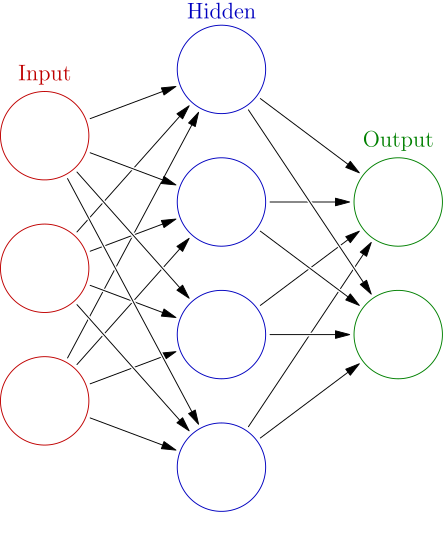
\includegraphics[width=0.25\textwidth]{nn_simple_1}~\caption{A simple Feed Forward Neural Network (FNN) with three layers: Input, Hidden and Output.\footnote{\cite{nn_simple_img_1}}}
        \label{fig:nn_simple_1}
    \end{figure}
    \noindent
    To describe the structure of a NN we also use the term topology.
    \begin{mydef}{Neural Network Topology}
        The topology of a neural network is its distinct arrangement of neurons, layers and the connections between the neurons.
        \label{definition:Topology}
    \end{mydef}
    \noindent
    For the neural network to perform functions, we also need to assign a weight to all connections.
    This weight value ranges from -1 to 1 and can be thought of as the strength of a connection between neurons.
    \\
    In terms of computer science, this structure now resembles a directed, weighted graph, which is why we will call the neurons nodes and their connections edges from now on.
    \begin{mydef}{Nodes/Edges}
        In a neural network, a node receives, computes and sends information, whereas an edge forms the connections between nodes to exchange information.
        \label{definition:Nodes-Edges}
    \end{mydef}
    \\ \\
    Now let's see, how information gets computed by a neural network by using the example of a computer vision NN, that recognizes digits on a black/white image:
    First, we need a way to encode the input image into values for the nodes of the input layer.
    In our example, we might use the Brightness values of the single pixels, which we directly assign to the nodes of the input layer.
    \\
    Then, for each node of the input layer, we look for all connected edges.
    For each of these edges we multiply its weight by the value of the input node and add the result to the node on the receiving end.
    \\
    After iterating through all the nodes of one layer, we move the next layer.
    At this point, the value of the nodes in this layer is the sum accumulated by the values of all connected nodes multiplied by the weight of that connection:
    \begin{equation}
        v_x = \sum_{i=0}^{N}v_i * w_i\label{eq:sum_connected_nodes}
    \end{equation}
    Where:
    \textit{
        \begin{itemize}
            \item N is the number of connected nodes
            \item $v_x$ is the value of the current node
            \item $v_i$ is the value of the connected node i
            \item $w_i$ is the weight of the edge connecting the current node to node i
        \end{itemize}
    }
    \noindent
    Additionally, we can add a bias value $r_x$ ranging from -1 to 1 onto the value of the nodes.
    Finally, an activation function $\sigma(x)$ is applied to the value of the nodes to fit the value of the node inside a preferred range.
    This activation function can also be thought of as the threshold of stimulation for a neuron to fire.
    Two examples for activation functions are:
    \begin{itemize}
        \item Sigmoid Function: $\sigma(x) = \frac{1}{1 + e^{-x}}$
        \item Rectified Linear Unit (ReLU): $\sigma(x) = \max{0, x}$
    \end{itemize}
    Plot of the activation functions:
    \\ \\
    \begin{center}
    \begin{tikzpicture}
     \begin{axis}[
     xmin=-6,
     xmax=6,
     ymin=0,
     ymax=6,
     ytick distance = 1,
     xtick distance = 1,
     minor tick num=1,
    axis lines = left,
    line width = 1.5pt,
    grid=both,
    major grid style={line width=0.8pt,draw=gray!50},
    minor grid style={line width=0.4pt,draw=gray!20},
    xlabel = \(x\),
    ylabel = {\(\sigma(x)\)}]
     \addplot[
        domain=-10:10,
        color=red,
        samples=1000.,
     ]{1/(1 + e^-x)};
\addlegendentry{\(Sigmoid\)}
     \addplot[
         domain=-10:10,
         color=blue,
         samples=1000.,
     ]{max(0,x)};
     \addlegendentry{\(ReLU\)}
     \end{axis}
    \end{tikzpicture}
    \end{center}
    \\ \\
    The complete function for the value of one node is therefore:
    \begin{equation}
        v_x = \sigma\left(\sum_{i=0}^{N}v_i * w_i + r_x\right)\label{eq:value_node}
    \end{equation}
    Where (additionally to equation~\ref{eq:sum_connected_nodes}):
    \textit{
        \begin{itemize}
            \item $r_x$ is the bias of the node
            \item $\sigma$ is the activation function
        \end{itemize}
    }
    \noindent
    Now this value $v_x$ is again sent through its connections to nodes from upcoming layers.
    After iterating through all the nodes and layers of the NN, we reach the final layer of the NN, where we can read out its computed output.
    This output again is encoded in node values like we did with the input and therefore needs to be decoded for the final result.
    In the example of a digit detecting NN, we could use 10 output nodes, each representing one digit.
    The result could be decoded by using the output node with the highest value as result.
    This kind of output encoding where all possible result get their own node is called one-hot encoding.
    With one-hot output encoding, the values of the output nodes can be interpreted as a certainty value for a specific result to be correct.
            \subsection{Remark: Functioning of NNs}\label{subsec:remark-about-the-funtioning-of-nns}
    Now that we have established how a NN works, it is important to understand why this kind of algorithm is revolutionary to computer science.
    \\ \\
    An algorithm processes an input with a set of functions applied in a certain order to calculate an output.
    Traditionally, a computer algorithm gets programmed with the help of mathematical operations, logic functions, loops, system functions and data structures, which are then converted into binary code for the processor.
    Of course, this also applies in the context of NNs, however, there is also a third layer of abstraction on top, which simulates the functioning of a brain with neurons.
    Since the traditional algorithm only enables the neurons of a NN, the third neuron-based layer is what computes the actual function of the NN\@.
    Therefore, NNs resemble more the functioning of a brain than a traditional algorithm.
    \\ \\
    This difference has implications for the functioning of an NN:
    Traditional algorithms represent actual mathematical calculations and are therefore deterministic.
    With NNs, the algorithm is based on different parameters for nodes and edges, which make it an unpredictable blackbox.
    In the top layer of abstraction, there are no concrete functions but only neuron activation that approximates a function instead.
    This means it is hard to prove a neural network to be always accurate and is also the reason why we often call the result of NNs its prediction.
    \begin{mydef}{NN Prediction}
        The output of a NN is called its prediction for some input.
    \end{mydef}
            \subsection{An Example of NN learning: Backpropagation}\label{subsec:an-example-of-nn-learning:-backpropagation}
    We already know how a NN with certain parameters can make a prediction for a given input.
    But how do we find such parameters encoding for the structure and weights/biases of the NN?
    The answer is to use machine learning, which trains the model to perform a certain task with the help of training data.
    \begin{mydef}{Machine Learning}
        Machine learning (ML) is a subset of artificial intelligence that involves the use of algorithms and statistical techniques to optimize artificially intelligent models for a given problem.
    \end{mydef}
    One machine learning algorithm for NNs is called backpropagation, which is one of the simplest and most efficient ways to train a NN.\@
    Backpropagation uses a training and test set containing unlabeled data for a problem.
    But what does a test set with unlabeled data mean in the context of machine learning?
    \begin{mydef}{(Un)labeled Data}
        Labeled data for a machine learning problem is a set of data with sample problems and the respective solutions.
        Unlabeled data instead only contains the sample problems.
    \end{mydef}
    The machine learning process of backpropagation starts with an NN with fixed topology and random weights/biases.
    First, the NN is given the training problems for which it will make random predictions.
    We will then refine these random predictions with the help of the sample solutions.
    This is done by looping back through the NN from the output layer to the input layer, always adjusting the weights and biases that the NN would finally make the right prediction for this problem.
    However, the NN shouldn't be adapted only to a single problem but make accurate predictions for the whole training set and unknown problems.
    To therefore prevent overcorrecting a NN for single problems, we have to factor in a learning rate that is significantly smaller than 1 for our correction.
    \\ \\
    The NN is trained on the whole training set for many generations, until the NN starts to make accurate predictions for all problems.
    To test the performance on unknown problems we can use a separate test set, which the NN wasn't trained on.

        \section{Evolutionary Computation (EC) \& Genetic Algorithms (GAs)}\label{sec:evolutionary-computation-(ec)-&-genetic-algorithms-(gas)}
    Now we will have a look at the Machine Learning Technique, this Thesis focuses on.
    Again, we will draw inspiration from Nature:
    \begin{mydef}{Evolutionary Computation}
    Evolutionary Computation (EC) is an Algorithm that optimizes a set of parameters for a problem with the help of natural selection.
    \end{mydef}
    EC is commonly used where the perfect parameters for some function can't be calculated but the performance of a certain set can be determined.
    One example scenario for EC might be if you have a large set of data points of an unknown polynomial function with noise and outliers.
    If you want to find the parameters for the underlying polynomial, you could then employ EC to find the best fitting parameters.
    Let's see how EC finds these parameters.
    \\ \\
    The process starts with an initial population of agents with random sets of parameters.
    EC then repeats following steps, forming a new generation of the population in each iteration:
    \begin{itemize}
        \item \textbf{Fitness evaluation:} First, EC needs to find out how good each agent with its parameters perform in the problem.
        We call the performance of an agent its fitness, which we either evaluate objectively with a cost function or relatively with a competition between agents.
        In our example, the cost function might check the prediction of the NN for the given data points, calculate its absolute differences to the values of the data points, and use the total sum as cost.
        \item \textbf{Selection:} As a next step, the agents that performed well are selected to be part of the next generation.
        \item \textbf{Reproduction:} The selected agents will then be replicated by directly copying their parameters (non-mating) or by merging parameters from different agents (crossover).
        \item \textbf{Mutation:} The agents parameters will then be mutated by either completely overwriting certain parameters with new random parameters or by shifting the existing parameters by a random number.
    \end{itemize}
    After a certain number of generations, you will then have the best performing set of parameters for a given problem.
    There is also one popular addition to EC, which draws inspiration from nature again:
    \begin{mydef}{Genetic Algorithm}
    A Genetic Algorithm (GA) is an implementation of EC that uses a genetic representation of the parameters.
    \end{mydef}
    Its main idea is to have genes that only encode indirectly for the parameters, and can be turned on or off.
            \subsection{Gradient Descent \& Local Minima}\label{subsec:gradient-descent}
    We know from the previous section that EC starts with an initial population of agents with random sets of parameters, which all have a fitness determined by the cost function.
    Agents with relatively low cost (or high fitness) survive the round and then get replicated a few times, mutated and again selected by cost.
    \\ \\
    This whole process strongly resembles a ball rolling down a hill in some terrain.
    On any given point on the terrain, the ball will roll down in the direction that goes down the steepest (we will disregard the inertia of the ball).
    If we apply this analogy to EC, the parameters for a function can be imagined as the horizontal coordinates for the ball meanwhile the cost of these parameters is the height at that location.
    The different mutations have parameters close to the original and can therefore be thought of as points close to the original in our terrain.
    As the ball rolls down to the lowest of all neighboring points in any moment, EC again chooses the set of parameters with the lowest cost every cycle.
    Because of this, our ML process is called gradient descent, as the algorithm evaluates all neighboring points and then follows the direction with the lowest cost and therefore steepest gradient.
    \\ \\
    So what does the ball analogy tell us about how EC learning works?
    Imagine a hill with each a shallow and a deep valley next to it.
    Depending on which side of the hill you place the ball in the beginning, it will roll in a different direction and end up in either of the two valleys, which have different heights.
    From this we can take away following things:
    \begin{itemize}
        \item (Minor) differences in the starting position can result in large differences in the end position and the respective cost.
        \item Once a point with no downwards gradient is reached, innovation halts for that agent, even if there is a point with lower cost somewhere else.
        Such points are called local minima.
    \end{itemize}
    \begin{mydef}{Local Minimum}
        A local minimum is a point with minimal cost compared to its neighboring area and is therefore a halting point for gradient descent.
    \end{mydef}
    The impact of starting position and local minima often pose a large problem for EC applications.
    Strategies to reduce the impact of such are therefore essential for the algorithms success.

        \section{Evolutionary Neural Networks (ENNs)}\label{sec:evolutionary-neural-networks-(enns)}
    After having covered all the basics about NNs and EC, we can now combine those concepts to create the algorithm this thesis is about.
    \begin{mydef}{Evolutionary Neural Networks}
        Evolutionary neural networks (ENNs) are neural networks that use evolutionary computation to optimize for its parameters for the NNs weights/biases and its topology.
    \end{mydef}
    ENNs are useful for complex machine learning problems and also work for unlabeled training data as long as there is a fitness function.
    Let's bring evolutionary computation into the context of neural networks:
    The parameters ENNs encode for are for the weights, biases, nodes and edges of a Neural Network.
    You could either directly encode the NNs parameters as a graph or indirectly as genes, which would make it a genetic algorithm.
    ENNs still start with a random population of agents that are evaluated and selected by a fitness function.
    Then they are replicated (with crossover or non-mating) and finally mutated in following ways:
    \begin{enumerate}
        \item \textbf{Change weights/biases:} A new random value is set for the weight or bias of a random existing edge or node.
        \item \textbf{Shift weights/biases:} The value for an existing weight or bias of a random existing edge or node is altered by a random change but is kept close to the old value.
        \item \textbf{Add edges:} A new edge is added between two random, previously unconnected nodes.
        \item \textbf{Add nodes:} A new node is added in between of a random existing edge.
        The old edge is removed and two new edges with random weights are added between the new node and the two other nodes each.
        \item \textbf{Remove nodes/edges:} A random node or edge is removed in a way that doesn't cut off the input from the output layer.
    \end{{enumerate}}
    \section{Drawing Inspiration from the NEAT-Apporach}\label{sec:drawing-inspiration-from-the-neat-apporach}
        As already stated in the thesis statement(\ref{sec:thesis-statement}), neuroevolution of augmenting topologies is a ENN machine learning algorithm developed by Kenneth O. Stanley and Risto Miikkulainen in 2002\footcite[p.105-106]{Neat_02}.
        One of its main innovations is that the initial population starts with NNs of lowest complexity and the NNs only increase topological complexity as its useful for the problem.
        In specific, we start with NNs that only have the nodes of the input layer connected to the nodes of the output layer.
        This should result in more efficient NNs for the problem as complexity is only increased when it improves the NNs performance.
        The NEAT algorithm therefore only needs the mutations 1. to 4. showed in the last section(\ref{sec:evolutionary-neural-networks-(enns)}) and doesn't need to remove complexity (mutation 5.) as it is already minimal.

    \section{Games}\label{sec:games}
    Let's also have a quick look at the games this Thesis will train the ENNs on.
    \subsection{Simple Nim}\label{subsec:simple-nim}
    This game is a simplified version of Nim, where two players take turns removing an arbitrary amount of matches from a single stack with some number of matches.
    The player who removes the last match loses.
    Therefore, the winning strategy simply is to remove all matches from the stack but one, which forces the opponent to remove the last match, which makes them lose.
    \subsection{Nim}\label{subsec:nim}
    This game works similarly to Simple Nim with the difference that there are multiple stacks with matches.
    Now, the player who removes the last match from the last unemptied stack loses.
    The winning strategy for Nim is much more complex, which forces the ENNs to learn a more complex strategy.
    You can read up the exact winning strategy on Wikipedia\footcite{nim_23} but the main point is that perfect play requires a complex algorithm.
    We won't expect the ENNs to learn this algorithm fully but hopefully they will be able to approximate perfect play that it can beat human players that don't know the perfect strategy.
    \section{Related Work}\label{sec:related-work}
    The field of AI research in ENNs is largely studied and is often linked to games.
    In the following table, we can find some examples of ENN models that have been tested on games:

    \footnotesize
    \begin{center}
        \hspace*{-2cm}\begin{tabular}{|| l l l l l ||}
          \hline
          \makecell{\textbf{Author(s) \& Year}} &
          \makecell{\textbf{Model}} &
          \makecell{\textbf{Game/Benchmark}} &
          \makecell{\textbf{Computation}} &
          \makecell{\textbf{Accuracy}} \\
          \hline\hline
          \makecell{\cite{Neat_02}} &
          \makecell{NEAT} &
          \makecell{Double Pole Balancing\\With Velocities} &
          \makecell{3600\\evaluations} &
          \makecell{100\%} \\
          \hline
          \makecell{\cite{dama_22}} &
          \makecell{NEAT} &
          \makecell{Dama} &
          \makecell{$>$5000\\generations} &
          \makecell{81.25\%\\(wins against humans)} \\
          \hline
          \makecell{\cite{go_98}} &
          \makecell{SANE} &
          \makecell{Go} &
          \makecell{260\\generations} &
          \makecell{$>$75\%\\(vs Wally, 9$\times$9 board)} \\
          \hline
          \makecell{\cite{capture_02}} &
          \makecell{Custom\\ENN} &
          \makecell{Capture Game\\(subgame of Go)} &
          \makecell{$>$100\\generations\\(distributed)} &
          \makecell{No significant\\progress yet} \\
          \hline
          \makecell{\cite{backgammon_07}} &
          \makecell{Genetic\\ENN} &
          \makecell{Backgammon} &
          \makecell{256 pop,\\100–200\\generations} &
          \makecell{62.4\%\\(vs Pubeval)} \\
          \hline
        \end{tabular}\hspace*{-2cm}
    \end{center}
    \normalsize
    Note:
    Although the amount of fitness evaluations is a more accurate representation of computation load than the amount of generations, in many cases the amount of fitness evaluations isn't indicated and cannot be derived.

    \chapter{Building my ENN}\label{ch:building-my-enn}

    \section{Algorithm Design}\label{sec:algorithm-design}
    Now, we will have a detailed look at how to use the concepts described in the last chapter(\ref{ch:introduction}) to build an evolutionary neural network that plays Nim.
    First, I will explain the general structure of my code:
        \subsection{Overview}\label{subsec:overview}
    As already mentioned in the thesis statement(\ref{sec:thesis-statement}), this project is written in the Rust programming language.
    If you don't understand the syntax of the code snippets, you can consult the online \("\)The Rust Programming Language\("\) booklet under: \url{https://doc.rust-lang.org/book/}
    \\ \\
    My codebase is divided into different modules as well as a bin folder with main files.
    The modules are divided into one module with the ENN algorithm, the other modules handle the different games, the ENNs learn to play.
    The ENN module is divided into two files:
    \begin{itemize}
        \item \textbf{agent.rs:} This file handles the NNs and the mutations on the NNs
        \item \textbf{population.rs:} This file handles the natural selection process and data saving
    \end{itemize}
    The game modules provide the problems for the NNs, handle the predictions of the NNs, and find the new game state after a move.
    It might also include an objective performance evaluation function to measure how well the NNs perform.
    I will now explain all the functions bottom up, starting with the neural network.
    I work with Rusts structs which are similar to classes in other programming languages.
            \subsection{Neural Network}\label{subsec:neural-network}
    The struct \textit{NeurualNetwork} (defined in agents.rs) most importantly contains a two-dimensional vector of nodes, which encodes all the information of the NN\@:
    \begin{minted}{rust}
    pub struct NeuralNetwork {
        [...] // redundant side data about the NN
        pub nodes: Vec<Vec<Node>>,
    }
    \end{minted}
    The vector inside (\mintinline{rust}{Vec<Node>}) represents a layer of the NN and the outside vector (\mintinline{rust}{Vec<Vec<Node>>}) contains all layers of the NN\@.
    A \textit{Node} contains its bias and a vector for the incoming and outgoing edges:
    \begin{minted}{rust}
    pub struct Node {
        pub bias: f64,
        //edges stored in an adjacency list
        pub incoming_edges: Vec<Edge>,
        pub outgoing_edges: Vec<Edge>,
    }
    \end{minted}
    An \textit{Edge} contains the weight of the edge and its input/output node:
    \begin{minted}{rust}
    pub struct Edge {
        input: [usize; 2],
        out: [usize; 2],
        weight: f64,
    }
    \end{minted}
    The most important functions of the \textit{NeuralNetwork} struct are:
    \begin{itemize}
        \item \mintinline{rust}{new(input_nodes: usize, output_nodes: usize) -> Self {}}, which initializes the NN with all input and output nodes connected to each other with random weights and biases.
        \item \mintinline{rust}{predict(&self, input: Vec<f64>) -> Vec<f64>}, which computes the output of the NN for a given input with the forward propagation algorithm described in~\ref{subsec:feed-forward-neural-networks-(fnns)}.
        \item \mintinline{rust}{activation_function(x: f64) -> f64}, which computes the neuron activation described in \ref{subsec:feed-forward-neural-networks-(fnns)}.
        We use a variant of the \texit{ReLU} function, since the linearity for inputs above 0 in the ReLU function allows for more variety of neuron activation, which makes the NN more flexible and efficient.
        The variant we use is the \texit{ELU} function, which additionally tackles the problem of dead neurons in \texit{ReLU} by allowing for negative values.
    \end{itemize}
            \subsection{Mutation}\label{subsec:mutation}
    The mutation of the NNs is handled in the \textit{Agent} struct (defined in agent.rs), which includes a NN, its fitness, and its rank:
    \begin{minted}{rust}
    pub struct Agent {
        pub nn: NeuralNetwork,
        pub fitness: f64,
        pub rank: isize,
    }
    \end{minted}
    The function \mintinline{rust}{mutate(&mut self, mutations: usize) -> Self {} } has a number of mutations as a parameter which it applies to the NN of the agent.
    For each mutation, it randomly selects one of the following mutations: Change weights/biases, Shift weights/biases, Add edges, Add nodes.
    All of these mutations have already been described in the last chapter(\ref{sec:evolutionary-neural-networks-(enns)}), although there are some implementation details to mention:
    \begin{itemize}
        \item When inserting a new node in between of two connected nodes (mutation 4.), the inserted node will be added to a random layer in between of the previously connected nodes.
        If the previously connected nodes are in neighboring layers, we create a new layer in between for the new node.
        \item The shift mutation adds to the initial value a random float in the range 0.0 to 1.0 squared with a random sign.
        This gives us following function: \\
        $v_{new} = shift(v_{old}) = v_{old} + rand(-1, 1) * rand_{float}(0..1)^2$
        \item The amount of mutations performed per NN is randomly selected in a range, which we can define as parameters (see section~\ref{subsec:enn-parameters}).
        \item The type of mutation that is performed is randomly determined for each mutation.
        We can also assign a weight to each mutation as parameters which represent its probability to be selected relatively to the weight of the other mutations (see again section~\ref{subsec:enn-parameters}).
    \end{itemize}

            \subsection{Evolutionary Computation}\label{subsec:natural-slection}
    The EC process starts with an initial population of agents with new, minimal NNs created by the \mintinline{rust}{NeuralNetwork::new()} function (described in \ref{subsec:neural-network}).
    As we already established before (see~\ref{sec:evolutionary-computation-(ec)-&-genetic-algorithms-(gas)}), we now repeat the steps of performance evaluation, selection and mutation.
                \subsubsection{Competition}
    In this case, the fitness evaluation works by letting the agents of a population compete against each other in the games.
    However, we can't let every agent play every other agent since the needed time increases quadratically with population size.
    My solution therefore is to use my circular pairing algorithm.
    This algorithm has a predefined number of opponents each agent needs to play against (see~\ref{subsec:enn-parameters}).
    For each of this predefined number of games, it generates a new distance which it then uses to pair each $\textrm{agent}_i$ with the $\textrm{agent}_{i+distance}$.
    It also checks that the distance isn't a multiple of any distance it had previously since this would result in the same agents being paired twice.
    Each game is played twice with both players starting once while keeping the same initial state.
                \subsubsection{Fitness Evaluation}
    Now, we need to evaluate the fitness of the agents with the fitness function.
    The main idea for the fitness function is to simply count the number of wins an agent has made during the competition.
    Of course, there are other possibilities to evaluate the performance of an agent that represent their performance more accurately.
    The reason why we still first try to use the number of wins as fitness is because it is a generally applicable function to any game.
    Counting the number of wins doesn't require a deeper understanding of the game, which is very useful in games that are indeterministic.
    This also enables the ENNs to find their own new strategy for the game, which is finally the goal of AI training.
                \subsubsection{Natural Selection}
    After the fitness evaluation, we can test the performance of the generation (details in section~\ref{subsec:performance-tests}) and then generate the new population.
    The new population is made up by some portion of each of the following:
    \begin{itemize}
        \item \textbf{Agents from the last generation:}
        The main part of the new population will be drawn from agents from the old generation with high fitness.
        This works by selecting all needed agents randomly using the fitness of our agents as their relative probability of being drawn.
        We can also raise the fitness to some power to either allow more or less survival of non top-performing agents.
        \item \textbf{Random agents from the last generation:}
        Some fraction of the new population is made up of randomly selected agents from the last generation which might help counter a population with the top performing agents stuck in local minimum.
        \item \textbf{New random agents:}
        Another fraction of the new population is made up of newly generated, random agents which might help counter overly complex NNs and also local minima in a population.
        \item \textbf{Old best agents:}
        The last part of the new population is made up of best agents from previous generations which help counter populations stuck in a local minimum.
    \end{itemize}
    Now that we have generated our new population, we can start over the whole process.
            \subsection{ENN Parameters}\label{subsec:enn-parameters}
    As already mentioned in the thesis statement(\ref{sec:thesis-statement}), my research involves testing my implementation with several configurations of different parameters and then evaluate their performance with the stats described in the following section(\ref{subsec:performance-tests}).
    Here is a list of all possible parameters influencing my ENNs:
    \begin{itemize}
        \item \textbf{General:} Size of the population
        \item \textbf{Game:} Initial state of the game, game function that encodes the state for the NN, decodes its prediction, and executes the move on the current state
        \item \textbf{Competition:} Number of opponents per agent
        \item \textbf{Selection:} Fitness exponent, share of old best agents, random agents from last generation and new random agents making up the new population besides agents selected by fitness
        \item \textbf{Mutation:} Min and max amount of mutations per agent, weight/probability of the different mutations
        \item \textbf{Evaluation:} Number of games from the best agent against old best agents

    \end{itemize}
    For each test, we then save a file with the information about the value of all these parameters.

    \subsection{Performance Tests}\label{subsec:performance-tests}
    To see how the Agents perform in the games, we need to track some stats and games.
    We save following data every generation after the competition phase:
    \begin{itemize}
        \item \textbf{Fitness of the best agent:} This stat shows us how much better the best agent performs relatively to the average agent.
        \item \textbf{Wins against older generations:} We pair the best agent against an evenly distributed set of the best agents from past generations to track relative performance to the past.
        As long as this number is above 50\%, we should expect improvement over older generations.
        \item \textbf{Objective grading:} This stat is the performance evaluation of the best agent based on some algorithm that either plays mathematically perfect or (in non-deterministic games) is generally accepted to play well.
        It is important to note that we primarily don't use this algorithm for the fitness function because of the points previously mentioned in section~\ref{subsec:natural-slection}.
        \item \textbf{Number of turns:} We track the average number of turns the agents needed while playing their competition games.
        In Nim, low turn count generally means better play.
        \item \textbf{Average amount of hidden layers and nodes per hidden layer:} We track these stats to see how complex the topologies of our NNs in the population are.
        \item \textbf{Best agent layer sizes and edges:} We track these topological stats to see how complex the best solution is.
        \item \textbf{Best agent games:} We track the whole games turn after turn played by the best agent from the current generation against each the best agent from the last generation and a randomly selected best agent from a previous generation.
        With these game logs, we can see what moves our agents make in real games and try to derive their tactics and strategies.
    \end{itemize}
            \subsection{Nim}\label{subsec:nim-implementation}
    For the nim game, there are a few different game modes as well as an objectively perfectly playing dynamic programming algorithm.
    Let's first look at the general idea of how a game is played.
                \subsubsection{General Approach}
    Each game starts with a first game state, which is derived from the initial state parameter.
    A game state is a list where its length is the amount of stacks in that game and each value $v_i$ stands for the amount of matches on the i-th stack.
    Then, the competing agents take turns predicting their moves.
    On their turn, the active agent reads the current game state as input and predicts its next move.
    A move indicates the stack where the matches are removed as well as the number of removed matches.
    Then the game function computes the new game state after the move or ends the game if all stacks are empty.

                \subsubsection{Encoding and Decoding}
    Our input is directly encoded into the input layer of the NNs, which means the input layer has the same size as the state.
    The values of the input nodes are directly copied from the game state list and therefore also represent the amount of matches on each stack.
    \\ \\
    For output encoding, there is two different implementations.
    \begin{itemize}
        \item \textbf{Direct encoding:} We have two output nodes where the value for the first represents the index of the stack and the second value represents the amount of matches that are removed.
        \item \textbf{One-hot encoding:} The first $N$ output nodes encode for the index and the following nodes encode for the amount of matches removed.
        For both the nodes encoding for index and amount removed, the node with the highest value is finally used as output.
        The output layer therefore has length $l = N + \max(state_{initial})$, where $N$ is the amount of stacks and $\max(state_{initial})$ is the highest possible amount of matches on a stack.
    \end{itemize}
    Direct encoding is the more straight forward approach with lower NN topology whereas one-hot encoding ensures that the output stays in a reasonable range.
                \subsubsection{Game Modes}
    There are game modes \texit{Simple Nim} and \texit{Nim} with some configuration possibilities:
    \\
    In \texit{Nim}, each stack of the initial state can hold matches whereas in Simple Nim, the value of all stacks but one randomly chosen stack is set to 0.
    \\
    The stack sizes in the initial state equal the corresponding values from the initial state parameter except for the configuration \textit{random}, where the stack sizes of the initial state are randomly selected with the corresponding values in the initial state parameter as upper bound.
    \\
    Another configuration involves the output decoding.
    With strict grading, illegal moves lead to a game loss, whereas in safe grading, the closest legal move to the illegal prediction is played.
                \subsubsection{Objective Grading}
    To have an exact measure of performance, we use a dynamic programming (DP) algorithm that knows the best moves for each given state.
    It works by first defining a base case, which in case of Nim is every stack being empty and the result a loss.
    Then, it starts with the initial state and tries out all possible moves using recursion.
    For each state it tries to find a move that forces the opponent into a losing position.
    If it can find such a move, the position is winning, but if all moves lead to winning position for the opponent, the algorithm returns the position with the maximal moves needed for the opponent to win.
    It also stores the result for each already computed state, so that all other paths that lead to that position can use the precomputed result.
    \\ \\
    Now that we know for all positions if they're winning, we can use this to grade the moves of our agents:
    For each move, an agent gets one point if
    \begin{itemize}
        \item the agent had a winning state and made a move that got the opponent into a losing state,
    \end{itemize}
    or if
    \begin{itemize}
        \item the agent had a losing state and made a move that required the maximal amount of moves for the opponent to win.
    \end{itemize}
    The sum of all points an agent has collected is then divided by the amount of moves it has made to get the final performance score.

    \section{Findings}\label{sec:first-findings}
    Now we will test our ENN algorithm with the games and different parameters.
    The general approach is to start by training the ENNs on easy problems whilst observing the effect of different parameters on the result.
    Each test is repeated at least 3 times to try to reduce the impact of randomness on the results.
    As we walk through the different testing configurations, we will discuss just one of the tests as long as all tests showed similar results.
    However, all testing data can be inspected on my GitHub.
            \subsection{Simple Nim}\label{subsec:simple-nim-results}
    For the Simple Nim game, I will run each test for 1000 generations, since ENNs should be able to solve this simple game rather quickly.
                \subsubsection{Stack: 2, Configuration 1}
    First we test the ENNs on a problem with one stack containing 2 matches.
    This is the easiest problem we can still consider a game - with one match on the stack there is only one legal move, so it doesn't involve much decision-making.
    The winning strategy of course is to only take one match and leave the opponent with the last match on the stack.
    We start our first test with a relatively small population of 100 agents and try to simplify all other parameters:
    \\
    \texttt{game function: run\_nim\_strict}, initial state: \texttt{[2]}, population size: \texttt{100}, competition games: \texttt{50}, mutation min: \texttt{0}, mutation max: \texttt{1}, fitness exponent: \texttt{1}, best agent share:
    \texttt{0}, random agent share: \texttt{0}, random old agent share: \texttt{0}, best agent tournament games: \texttt{50}, add\_connection\_rand: \texttt{1}, add\_node\_rand: \texttt{1}, change\_weight\_rand: \texttt{1}, change\_bias\_rand: \texttt{1}, shift\_weight\_rand: \texttt{1}, shift\_bias\_rand: \texttt{1}\\
    It is also important to note that we start with one-hot output encoding, since this means that the output stays in the desired range.
    \\ \\
    Now, we'll run it and see how it goes:
    \\
    \newcommand{\csvpath}{../data/simple_nim/stack_2/t_1/stats.csv} % Rename the macro
    \begin{center}
        \begin{tikzpicture}
            \begin{axis} [
                grid=both,
                xmin=0,
                xmax=50,
                ymin=0,
                ymax=150,
                no markers,
                xtick distance = 10,
                ytick distance = 25,
                legend pos=north west, % Adjust legend position
                xlabel={Generation},
                ylabel={Performance},
            ]
                \caption{Performance of the best agent over generations.}
                \label{fig:sn_stack_1_t_1}
                % First plot
                \addplot table [
                x=generation,
                y=best_agent_avg_performance,
                col sep=comma,
                ] {\csvpath};
                \addlegendentry{\( \text{Best agent perfect play \% (accuracy)} \)}

                % Second plot
                \addplot table [
                x=generation,
                y=best_agent_wins_percentage,
                col sep=comma,
                ] {\csvpath};
                \addlegendentry{\( \text{Best agent wins \%} \)}
            \end{axis}
        \end{tikzpicture}
    \end{center}

    As we can see, the best agent already plays the game perfectly after one generation.
    We can also observe this in our saved games, where the best agent correctly plays the move [0, 1] (first value is the stack, second value the number of matches removed):
    \begin{minted}{}
    Generation: 1
    Best agent layer sizes: [1, 3]
    Agent 1 vs Agent 0:
    Turn: 0: state: [2], agent_move: [0, 1]
    Turn: 1: state: [1], agent_move: [0, 1]
    Game result: [1, 0]
    \end{minted}
    The best agent wins percentage in the plot above is a steady 50\% since all games are played both ways and the first agent always wins the game.
            \subsubsection{Stack: 8, Configuration 1}
    Since the stack size with 2 has already worked fine, we will now try the same configuration with an increased initial stack size of 8 matches:
    \\
    \renewcommand{\csvpath}{../data/simple_nim/stack_8/t_1/stats.csv} % Rename the macro
    \begin{center}
        \begin{tikzpicture}
            \begin{axis} [
                grid=both,
                xmin=0,
                xmax=1000,
                ymin=0,
                ymax=150,
                no markers,
                xtick distance = 200,
                ytick distance = 25,
                legend pos=north west, % Adjust legend position
                xlabel={Generation},
                ylabel={Performance},
            ]
                \caption{Performance of the best agent over generations.}
                \label{fig:sn_stack_8_t_1}
                % First plot
                \addplot table [
                x=generation,
                y=best_agent_avg_performance,
                col sep=comma,
                ] {\csvpath};
                \addlegendentry{\( \text{Best agent perfect play \% (accuracy)} \)}

                % Second plot
                \addplot table [
                x=generation,
                y=best_agent_wins_percentage,
                col sep=comma,
                ] {\csvpath};
                \addlegendentry{\( \text{Best agent wins \%} \)}
            \end{axis}
        \end{tikzpicture}
    \end{center}
    The accuracy of the runs got up to around 30\% and if we look at the games recorded in generation 982, we can see why it didn't get to 100\%.
    \begin{minted}{}
    Agent 998 vs Agent 999:
    Turn: 0: state: [8], agent_move: [0, 2]
    Turn: 1: state: [6], agent_move: [0, 2]
    Turn: 2: state: [4], agent_move: [0, 2]
    Turn: 3: state: [2], agent_move: [0, 1]
    Turn: 4: state: [1], agent_move: [0, 3]
    \end{minted}
    The best agent only learned to play the moves where it subtracts one or two matches.
    This seems quite bad since seemingly all the NNs have to do is to play [0, 7] instantly.
    So why couldn't it learn this one move, when it could do it with stack size 2?
    The problem is that if the starting player subtracts less than 7 matches, the other player would get in winning position where it has to adapt and play subtract N - 1 matches.
    There might evolve a population where all agents only subtract 7 matches, however this seems more like a local minimum and our final goal is to develop NNs that can play the whole game.
    This simplification turns out to be a hindrance, so we will change the stack to have a variable amount of matches.
    \subsubsection{Remark: Unnecessary Topology}
    If we look at the topology metrics of one of the tests, we realize that complexity of the NNs exploded without any visible improvement in performance:
    \begin{center}
        \begin{tikzpicture}
            \begin{axis}[
                title=\textbf{Topology},
                grid=both,
                xmin=0, xmax=1000,
                ymin=0, ymax=50,
                no markers,
                xtick distance = 200,
                ytick distance = 10,
                legend pos=north west,
                xlabel={Generation},
                ylabel={Complexity},
            ]
                \addplot[violet] table [
                x=generation,
                y=avg_layers,
                col sep=comma,
                ] {\csvpath};
                \addlegendentry{Average layers}
                \addplot[teal] table [
                x=generation,
                y=avg_hidden_layer_size,
                col sep=comma,
                ] {\csvpath};
                \addlegendentry{Average hidden layer size}
            \end{axis}
        \end{tikzpicture}
    \end{center}
    We get an average amount of over 20 hidden layers with on average 2 nodes.
    It doesn't make sense for the NNs to have such complexity for such a simple problem as it only increases the needed computations.
    We will therefore reduce the chance for a new nodes and edges to form by a factor of 20 each.
    Let's see if this change impacted the performance and topology of the NNs:
    \\
    \begin{figure}[H]

        \centering
        \pgfplotsset{width=9.5cm,height=6cm,compat=1.18}
        % First graph
        \begin{adjustbox}{valign=c,margin=-2cm 0pt 0pt 0pt} % Shift content left by 2cm
            \begin{minipage}{1.1\textwidth}
                \begin{subfigure}[b]{0.45\textwidth}
                    \centering
                    \begin{tikzpicture}
                        \renewcommand{\csvpath}{../data/simple_nim/stack_8/t_1x/stats.csv} % Rename the macro
                        \begin{axis}[
                            title=\textbf{Performance},
                            grid=both,
                            xmin=0, xmax=1000,
                            ymin=0, ymax=150,
                            no markers,
                            xtick distance = 200,
                            ytick distance = 25,
                            legend pos=north west,
                            xlabel={Generation},
                            ylabel={Performance},
                        ]
                            \addplot table [
                            x=generation,
                            y=best_agent_avg_performance,
                            col sep=comma,
                            ] {\csvpath};
                            \addlegendentry{Best agent perfect play \% (accuracy)}
                            \addplot table [
                            x=generation,
                            y=best_agent_wins_percentage,
                            col sep=comma,
                            ] {\csvpath};
                            \addlegendentry{\( \text{Best agent wins \%} \)}
                        \end{axis}
                    \end{tikzpicture}
                \end{subfigure}
                \hfill
                % Second graph
                \begin{subfigure}[b]{0.45\textwidth}
                    \centering
                    \begin{tikzpicture}
                        \renewcommand{\csvpath}{../data/simple_nim/stack_8/t_1x/stats.csv} % Rename the macro
                        \begin{axis}[
                        title=\textbf{Topology},
                        grid=both,
                        xmin=0, xmax=1000,
                        ymin=0, ymax=50,
                        no markers,
                        xtick distance = 200,
                        ytick distance = 10,
                        legend pos=north west,
                        xlabel={Generation},
                        ylabel={Complexity},
                        ]
                        \addplot[violet] table [
                        x=generation,
                        y=avg_layers,
                        col sep=comma,
                        ] {\csvpath};
                        \addlegendentry{Average layers}
                        \addplot[teal] table [
                        x=generation,
                        y=avg_hidden_layer_size,
                        col sep=comma,
                        ] {\csvpath};
                        \addlegendentry{Average hidden layer size}
                        \end{axis}
                    \end{tikzpicture}
                \end{subfigure}

            \end{minipage}
        \end{adjustbox}
        \caption{Performance metrics over generations in a 2x2 grid.}
        \label{fig:performances-1}
    \end{figure}
    \\
    Our modifications didn't impact the performance of the NN, but definitely helped keeping the topological complexity in a reasonable bound.
    We will keep these modifications moving on.

    \subsubsection{Stack 1--8, Configuration 1}
    We will repeat the previous test but with a variable amount of matches between 1 and 8:
    \renewcommand{\csvpath}{../data/simple_nim/stack_8r/t_1.2/stats.csv} % Rename the macro
    \begin{center}
        \begin{tikzpicture}
            \begin{axis} [
                grid=both,
                xmin=0,
                xmax=1000,
                ymin=0,
                ymax=150,
                no markers,
                xtick distance = 200,
                ytick distance = 25,
                legend pos=north west, % Adjust legend position
                xlabel={Generation},
                ylabel={Performance},
            ]
                \caption{Performance of the best agent over generations.}
                \label{fig:sn_stack_8r_t_1.1}
                % First plot
                \addplot table [
                x=generation,
                y=best_agent_avg_performance,
                col sep=comma,
                ] {\csvpath};
                \addlegendentry{\( \text{Best agent perfect play \% (accuracy)} \)}

                % Second plot
                \addplot table [
                x=generation,
                y=best_agent_wins_percentage,
                col sep=comma,
                ] {\csvpath};
                \addlegendentry{\( \text{Best agent wins \%} \)}
            \end{axis}
        \end{tikzpicture}
    \end{center}
    In my tests, the best agent perfect play performance always reaches a value ranging from 40\% to 75\% where it remained stable.
    The NNs were only able to learn the moves where they subtract 1, 2 and 3 matches but no others.
    \begin{minted}{}
    Agent 998 vs Agent 999:
    Turn: 0: state: [6], agent_move: [0, 3]
    Turn: 1: state: [3], agent_move: [0, 2]
    Turn: 2: state: [1], agent_move: [0, 1]
    \end{minted}
    The performance of NNs in different tests just depended on how many moves the NNs learned.
    In any case however, the NNs have got stuck in a local minimum.
    Such local minima originate in an early generations where the agents aren't highly developed, which means they often only play one move.
    The agents that only subtracted one match were therefore the most successful and reproduced the most.
    After reaching that local minimum, there wasn't a competitor that could assert itself, either because of a flaw in the selection process or because none were created in first place.
    We can also see how homogeneous the NNs across generations have become by looking at the wins of the best agent against former best agents, which always settles at 50\%, revealing that they all use the same strategy.
    We will therefore try to modify some parameters to see if anything helps against such local minima.

    \subsubsection{Stack 1--8, Configuration 2--5}
    To overcome local minima, we can use following strategies:
    \begin{itemize}
        \item \textbf{Fitness Exponent:} Increasing the fitness exponent to \textit{ex.} 2 might help successful mutations reproduce better and therefore overcome a large population of similar NNs.
        \item \textbf{Population Composition:} We can add other kinds of agents to the new population like best agents from older generations, randomly selected agents from the last generation, or newly generated random agents.
        This might help the development of new and possibly more complex strategies without the need for instant return in performance.
        \item \textbf{Population Size:} A larger population means more agents with different strategies can exist, evolve and finally help overcoming local minima.
    \end{itemize}
    We now test the effect of these parameters with following 4 configurations:
    \begin{enumerate}
        \item Fitness exponent set to 2
        \item Old best agents, random agents, and new agents each make up 15\% of the population
        \item Population size set to 2500
        \item All parameters combined
    \end{enumerate}
    \begin{figure}[H]

        \centering
        \pgfplotsset{width=9.5cm,height=6cm,compat=1.18}
        % First graph
        \begin{adjustbox}{valign=c,margin=-2cm 0pt 0pt 0pt} % Shift content left by 2cm
            \begin{minipage}{1.1\textwidth}
                \begin{subfigure}[b]{0.45\textwidth}
                    \centering
                    \begin{tikzpicture}
                        \renewcommand{\csvpath}{../data/simple_nim/stack_8r/t_2/stats.csv} % Rename the macro
                        \begin{axis}[
                            title=\textbf{Fitness exponent: 2},
                            grid=both,
                            xmin=0, xmax=1000,
                            ymin=0, ymax=150,
                            no markers,
                            xtick distance = 200,
                            ytick distance = 25,
                            legend pos=north west,
                            xlabel={Generation},
                            ylabel={Performance},
                        ]
                            \addplot table [
                            x=generation,
                            y=best_agent_avg_performance,
                            col sep=comma,
                            ] {\csvpath};
                            \addlegendentry{Best agent perfect play \% (accuracy)}
                            \addplot table [
                            x=generation,
                            y=best_agent_wins_percentage,
                            col sep=comma,
                            ] {\csvpath};
                            \addlegendentry{\( \text{Best agent wins \%} \)}
                        \end{axis}
                    \end{tikzpicture}
                \end{subfigure}
                \hfill
                % Second graph
                \begin{subfigure}[b]{0.45\textwidth}
                    \centering
                    \renewcommand{\csvpath}{../data/simple_nim/stack_8r/t_3/stats.csv} % Rename the macro

                    \begin{tikzpicture}
                        \begin{axis}[
                            title=\textbf{New population composition (each 15\%)},
                            grid=both,
                            xmin=0, xmax=1000,
                            ymin=0, ymax=150,
                            no markers,
                            xtick distance = 200,
                            ytick distance = 25,
                            legend pos=north west,
                            xlabel={Generation},
                            ylabel={Performance},
                        ]
                            \addplot table [
                            x=generation,
                            y=best_agent_avg_performance,
                            col sep=comma,
                            ] {\csvpath};
                            \addlegendentry{Best agent perfect play \% (accuracy)}
                            \addplot table [
                            x=generation,
                            y=best_agent_wins_percentage,
                            col sep=comma,
                            ] {\csvpath};
                            \addlegendentry{\( \text{Best agent wins \%} \)}
                        \end{axis}
                    \end{tikzpicture}
                \end{subfigure}

                \vspace{1em}

                % Third graph
                \begin{subfigure}[b]{0.45\textwidth}
                    \centering
                    \begin{tikzpicture}
                        \renewcommand{\csvpath}{../data/simple_nim/stack_8r/t_4/stats.csv} % Rename the macro

                        \begin{axis}[
                            title=\textbf{Population size: 2500},
                            grid=both,
                            xmin=0, xmax=1000,
                            ymin=0, ymax=150,
                            no markers,
                            xtick distance = 200,
                            ytick distance = 25,
                            legend pos=north west,
                            xlabel={Generation},
                            ylabel={Performance},
                        ]
                            \addplot table [
                            x=generation,
                            y=best_agent_avg_performance,
                            col sep=comma,
                            ] {\csvpath};
                            \addlegendentry{Best agent perfect play \% (accuracy)}
                            \addplot table [
                            x=generation,
                            y=best_agent_wins_percentage,
                            col sep=comma,
                            ] {\csvpath};
                            \addlegendentry{\( \text{Best agent wins \%} \)}
                        \end{axis}
                    \end{tikzpicture}
                \end{subfigure}
                \hfill
                % Fourth graph
                \begin{subfigure}[b]{0.45\textwidth}
                    \centering
                    \begin{tikzpicture}
                        \renewcommand{\csvpath}{../data/simple_nim/stack_8r/t_5/stats.csv} % Rename the macro

                        \begin{axis}[
                            title=\textbf{All combined},
                            grid=both,
                            xmin=0, xmax=1000,
                            ymin=0, ymax=150,
                            no markers,
                            xtick distance = 200,
                            ytick distance = 25,
                            legend pos=north west,
                            xlabel={Generation},
                            ylabel={Performance},
                        ]
                            \addplot table [
                            x=generation,
                            y=best_agent_avg_performance,
                            col sep=comma,
                            ] {\csvpath};
                            \addlegendentry{Best agent perfect play \% (accuracy)}
                            \addplot table [
                            x=generation,
                            y=best_agent_wins_percentage,
                            col sep=comma,
                            ] {\csvpath};
                            \addlegendentry{\( \text{Best agent wins \%} \)}
                        \end{axis}
                    \end{tikzpicture}
                \end{subfigure}


            \end{minipage}
        \end{adjustbox}
        \caption{Performance metrics over generations in a 2x2 grid.}
        \label{fig:performances-2}


    \end{figure}
    As we can see in the graphs, the performance didn't reach 100\% in any configuration and the NNs remained stuck in a local minimum with the best agents always winning 50\% against previous best agents.
    However, there is still something we can change.
                \subsubsection{Stack 1--8, Configuration 6}
    We run the simple configuration as in configuration 1, only that we changed the output encoding (explained in chapter~\ref{subsec:nim-implementation}) from one-hot to direct encoding:
    \\
    \renewcommand{\csvpath}{../data/simple_nim/stack_8r/t_6/stats.csv} % Rename the macro
    \begin{center}
        \begin{tikzpicture}
            \begin{axis} [
                grid=both,
                xmin=0,
                xmax=1000,
                ymin=0,
                ymax=150,
                no markers,
                xtick distance = 200,
                ytick distance = 25,
                legend pos=north west, % Adjust legend position
                xlabel={Generation},
                ylabel={Performance},
            ]
                \caption{Performance of the best agent over generations.}
                \label{fig:sn_stack_8r_t_2}
                % First plot
                \addplot table [
                x=generation,
                y=best_agent_avg_performance,
                col sep=comma,
                ] {\csvpath};
                \addlegendentry{\( \text{Best agent perfect play \% (accuracy)} \)}

                % Second plot
                \addplot table [
                x=generation,
                y=best_agent_wins_percentage,
                col sep=comma,
                ] {\csvpath};
                \addlegendentry{\( \text{Best agent wins \%} \)}
            \end{axis}
        \end{tikzpicture}
    \end{center}
    Now finally got it working!
    The best agent's performance reaches 100\% after 13 generations.
    \\
    So why did the change of output encoding affect the result that heavily?
    \\ \\
    If we look at the NN structure we had a single output neuron for each possible amount of matches we can subtract in one-hot encoding.
    During the evolution process, the connections to the neurons for output 1 and 2 got stronger than the other ones since it lead to a competitive advantage.
    This unfortunately also meant, that the NN was practically unable to adapt to activate the other output neurons.
    In fact, this behaviour would have been entirely predictable, since there is no mathematical way to model an NN that solves this problem with one-hot encoding except for NNs with large amount of hidden nodes.
    Yet NNs with large amount of hidden nodes are unlikely to develop with my ENNs since they don't show a competitive advantage instantly.
    \subsection{Nim}
    We now already have gained a lot of insight about the functioning of ENNs and are therefore ready for the normal version of Nim.

            \section{Direct Comparisons}
    \chapter{Wrapping Up}
        \section{Auto Review}
        \section{Future Work}
    \chapter{Appendix}
        \section{Code}
        \section{Data}
        \section{Documentation}
        \section{References}
    \printbibliography

\end{document}
